\chapter{Aufgabe 1}

\section{a)}

Die Zeitlinien für die verschiedenen Schedulestrategien \textit{SJF}, \textit{RR100} und \textit{RR50} sind in der Abbildung~\ref{fig:zeitlinie} dargestellt.\\
Auf den Zeitlinien ist jeweils der Zeitpunkt vermerkt, wann zu den jeweiligen Prozessen umgeschaltet wird (relativ zum Startzeitpunkt $0$ unter Berücksichtigung der Umschaltzeiten).
Die Gesamtlaufzeiten der einzelnen Verfahren für die geg. Prozesse sind an den Enden der Zeitlinien vermerkt.\\

\noindent
Es zeigt sich, dass \textit{SJF} eine effiziente Strategie für die Zuteilung von CPU-Zeit für die gegebenen Prozesse wäre, allerdings weist \textit{Mandl} auf die Unlösbarkeit der Frage hin, wie das Betriebssystem herausfindet, wieviel Zeit ein Prozess benötigt\footnote{
vgl. hierzu das \textit{Halteproblem} in der theoretischen Informatik, das - informell - besagt, dass es kein algorithmisches Verfahren gibt, mit dem bestimmt werden kann, ob die Ausführung eines Programms in endlicher Zeit stoppt (vgl.~\cite[363 ff.]{VW16j}). Relevant ist dies bspw. mathematischen Problemen wie der \textit{Collatz-Vermutung}.
}, weshalb SJF in der Praxis so kaum anwendbar ist (vgl.~\cite[104]{Man20f})

\begin{figure}
    \centering
    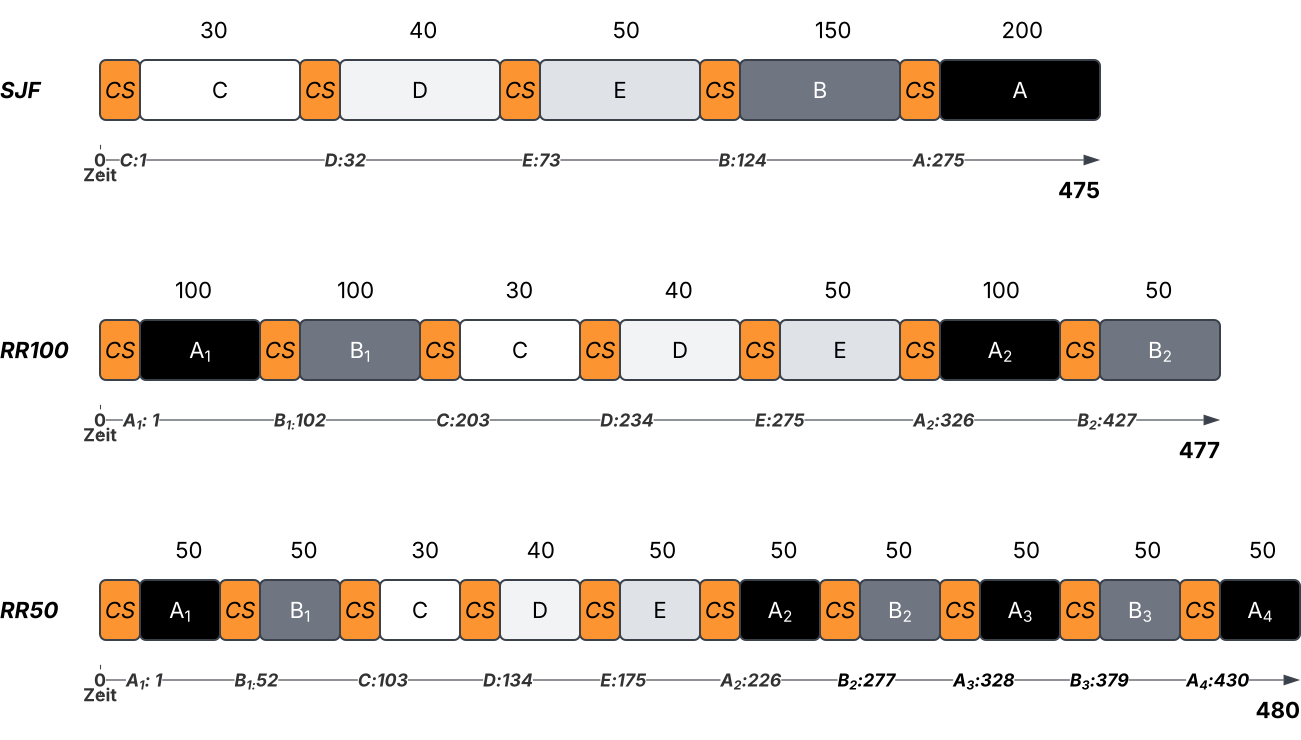
\includegraphics[scale=0.35]{aufgabe 1/img/zeitlinie.svg}
    \caption{Zeitlinien für die verschiedenen Schedulestrategien \textit{SJF}, \textit{RR100} und \textit{RR50} (nicht maßstabsgetreu). Prozesse mit dunkleren Farben nehmen viel CPU-Zeit in Anspruch. Der Kontextwechsel ist orange markiert (CS = \textit{Context Switch}). (Quelle: eigene)}
    \label{fig:zeitlinie}
\end{figure}

\section{b)}

Die jeweiligen Verweilzeiten\footnote{
auch: \textit{Turnaround-Zeit}, also \textit{gesamte Zeit}, in der sich ein Prozess im System befindet (vgl. \cite[108]{Man20f})
}der Prozesse sind in Tabelle~\ref{tab:verweilzeiten} angegeben.\\

\noindent
Die Herleitung der mittleren Verweilzeiten sind wie folgt hergeleitet:

\begin{equation}\notag
\begin{alignat}{3}
    \text{VZ}_{\text{SJF}} &= \frac{ \text{VZ}^\text{SJF}_A +  \text{VZ}^\text{SJF}_B +  \text{VZ}^\text{SJF}_C + \text{VZ}^\text{SJF}_D + \text{VZ}^\text{SJF}_E }{5} &&= 195 \text{ms} \\
    \text{VZ}_{\text{RR100}} &= \frac{ \text{VZ}^\text{RR100}_A +  \text{VZ}^\text{RR100}_B +  \text{VZ}^\text{RR100}_C + \text{VZ}^\text{RR100}_D + \text{VZ}^\text{RR100}_E }{5} &&= 347 \text{ms}  \\
    \text{VZ}_{\text{RR50}} &= \frac{ \text{VZ}^\text{RR50}_A +  \text{VZ}^\text{RR50}_B +  \text{VZ}^\text{RR50}_C + \text{VZ}^\text{RR50}_D + \text{VZ}^\text{RR50}_E }{5} &&= 288.2 \text{ms}
\end{alignat}
 \end{equation}


\begin{table}[h]
    \centering
    \setlength{\tabcolsep}{0.5em}
    \def\arraystretch{1.5}
    \begin{tabular}{|l|c|c|c|c|c|c|c|}
        \hline
        \textbf{Strategie} & $\text{VZ}_A$ & $\text{VZ}_B$ & $\text{VZ}_C$ & $\text{VZ}_D$ & $\text{VZ}_E$ & \textbf{mittlere VZ} & \textbf{Umschaltzeiten} \\
        \hline
        SJF      &     $475$    &    $274$     &     $31$    &     $72$    &     $123$    &         $195$                &            $5$      \\ \hline
        RR100    &   $426$      &     $477$    &    $233$     &    $274$     &    $325$     &          $347$               &              $7$     \\ \hline
        RR50     &    $480$     &    $429$     &    $133$     &     $174$    &    $225$     &          $288.2$              &             $10$       \\
        \hline
    \end{tabular}
    \caption{Verweilzeiten (VZ) der Prozesse bei den verschiedenen Scheduling-Strategien. Angaben in \textit{ms}
    \label{tab:verweilzeiten} (millisekunden).}
\end{table}